\chapter{Engineering Practices for AI-Native Teams}
\label{ch:ai-native-teams}

\begin{quote}
\itshape
``The team that ships AI-powered features fastest isn't the team with the best models. It's the team with the best engineering practices around those models.''
\end{quote}

\vspace{0.5cm}

\noindent
The previous chapter covered AI-assisted \emph{development}---how individual developers use AI tools to write code. This chapter zooms out to the team level: how engineering organizations must restructure their practices, roles, and workflows for a world where AI is not a tool bolted onto existing processes but a core collaborator embedded in every stage of the software development lifecycle.

The shift from ``AI-assisted'' to ``AI-native'' is not merely semantic. An AI-assisted team uses Copilot to autocomplete code. An AI-native team designs its entire workflow around human-AI collaboration: architecture documents are structured for AI consumption, code review processes account for AI-generated contributions, testing strategies address the unique failure modes of probabilistic systems, and team structures reflect the reality that a small group of senior engineers with AI leverage can outperform a large team without it.


\section{The New Team Structure: Centaur Pods}

The traditional software team---8 to 12 engineers with a mix of junior, mid-level, and senior---is giving way to smaller, senior-weighted teams that AI amplifies. Figure~\ref{fig:centaur-pod} contrasts the two models.

\begin{figure}[htbp]
\centering
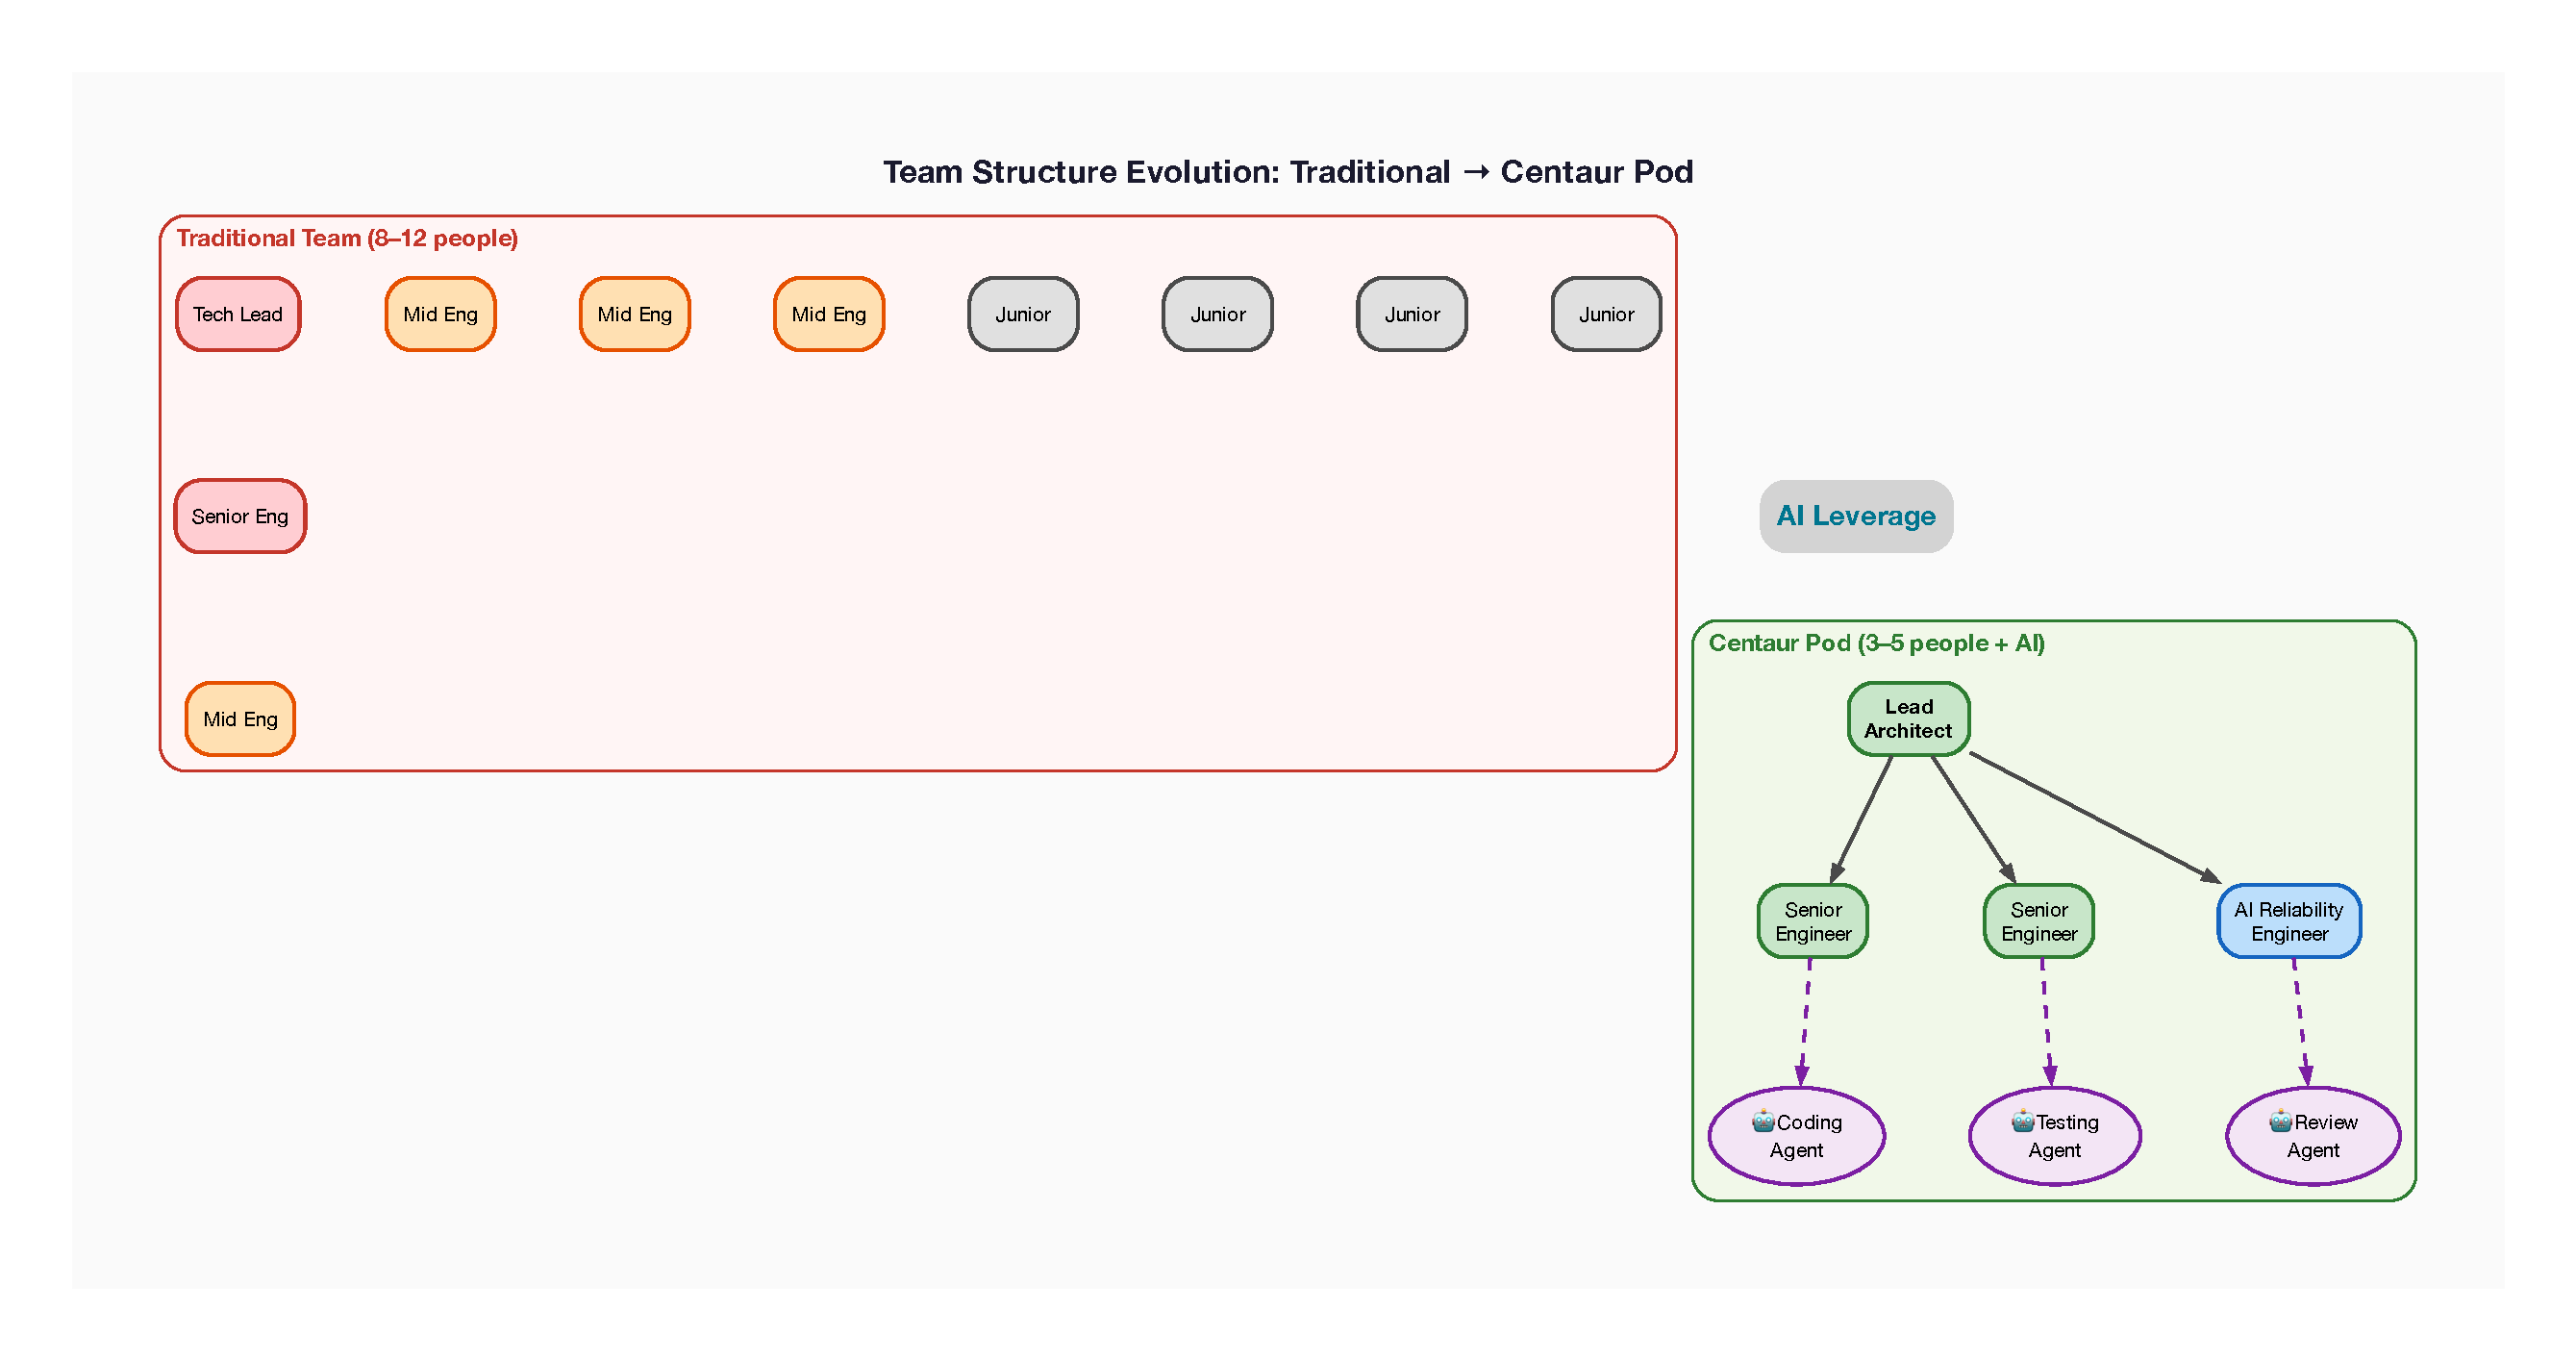
\includegraphics[width=\textwidth]{diagrams/compiled/ch10/centaur-pod.pdf}
\caption{Team structure evolution: from traditional 8--12 person teams to AI-augmented Centaur Pods}
\label{fig:centaur-pod}
\end{figure}

\subsection{Why Smaller Teams Win}

AI coding tools disproportionately amplify senior engineers. A senior engineer with deep architectural knowledge and strong AI fluency can now produce the implementation output of three to four engineers. This changes the optimal team composition:

\begin{table}[htbp]
\centering
\caption{Team structure evolution: traditional vs. AI-native}
\label{tab:team-evolution}
\begin{tabularx}{\textwidth}{lXX}
\toprule
\textbf{Dimension} & \textbf{Traditional (Pre-AI)} & \textbf{AI-Native (2026)} \\
\midrule
Team size & 8--12 members & 3--5 members (``Centaur Pod'') \\
Seniority mix & 2 senior, 4 mid, 4--6 junior & 2--3 senior, 1--2 mid, AI agents \\
Primary output & Code (PRs per week) & Shipped features per week \\
Bottleneck & Implementation speed & Design quality \& review bandwidth \\
Junior role & Apprentice (learning by implementing) & AI reliability engineer (learning by validating) \\
Knowledge capture & Tribal knowledge, onboarding docs & Codified in project context files \\
\bottomrule
\end{tabularx}
\end{table}

The ``Centaur Pod'' model---named after the human-AI hybrid chess teams that outperform both pure humans and pure machines---typically consists of:

\begin{itemize}[leftmargin=*]
    \item \textbf{Lead Architect} (1): Owns the system design, makes technology choices, and defines the constraints that AI agents operate within
    \item \textbf{Senior Engineers} (1--2): Implement features using AI tools, review AI-generated code, and handle the complex work that AI cannot reliably do (security, distributed systems, performance optimization)
    \item \textbf{AI Reliability Engineer} (1): A new role that combines quality assurance, security review, and AI governance. This person validates AI-generated output, maintains evaluation suites, and ensures that the team's AI workflow doesn't accumulate technical debt
\end{itemize}

\begin{cautionbox}[The Junior Developer Gap]
Smaller, senior-heavy teams raise a genuine concern: how do junior developers learn if AI handles the implementation work they traditionally used to do? The answer is evolving. Junior engineers in AI-native teams learn by validating AI output rather than writing code from scratch---they develop judgment and architectural thinking faster, but may develop weaker ``from-scratch'' coding skills. Teams must deliberately create learning opportunities that build foundational skills.
\end{cautionbox}


\section{New Roles in AI-Native Engineering}

\subsection{The AI Reliability Engineer}

The most important new role. The AI Reliability Engineer (AIRE) is responsible for ensuring that AI-generated code meets production quality standards. Their responsibilities include:

\begin{itemize}[leftmargin=*]
    \item Maintaining and evolving evaluation suites for AI-generated code
    \item Running security audits on AI-generated contributions
    \item Monitoring AI tool usage patterns and identifying misuse or over-reliance
    \item Managing project context files and ensuring they remain accurate
    \item Tracking and reporting on AI-assisted development metrics
\end{itemize}

\subsection{The AI Orchestrator}

In teams that use multi-agent workflows, the AI Orchestrator designs and manages the agent pipelines:

\begin{itemize}[leftmargin=*]
    \item Defining which agents handle which tasks
    \item Setting up the constraint systems (guardrails, approval gates, budget limits)
    \item Debugging agent failures---when an agent enters a loop, produces incorrect output, or exceeds its budget
    \item Optimizing the cost/quality tradeoff across different agent configurations
\end{itemize}

\subsection{The Product-Engineer Hybrid}

As AI lowers the barrier to implementation, the line between product management and engineering blurs. Engineers who deeply understand user needs can prototype, build, and iterate on features without waiting for a product spec. This ``product-minded engineer'' is increasingly valued:

\begin{itemize}[leftmargin=*]
    \item Can translate user problems directly into working prototypes using AI tools
    \item Makes product decisions informed by technical feasibility
    \item Reduces the communication overhead between product and engineering teams
    \item Enables faster iteration cycles (idea $\to$ prototype in hours, not weeks)
\end{itemize}


\section{Engineering Practices That Change}

\subsection{Code Review in an AI-Native World}

Code review is more important in an AI-native team, not less. When a significant portion of code is AI-generated, the reviewer's job shifts:

\begin{itemize}[leftmargin=*]
    \item \textbf{From syntax to semantics}: Less time checking formatting and variable names (AI gets these right), more time checking architectural alignment and business logic correctness
    \item \textbf{From completeness to correctness}: AI-generated code is usually ``complete'' but may have subtle incorrectness. Reviewers must focus on edge cases, error handling, and security
    \item \textbf{From individual PRs to patterns}: Watch for architectural drift---AI tools tend to implement the simplest solution, which may not be the right solution for your system's long-term health
\end{itemize}

\subsection{Documentation as a First-Class Artifact}

In AI-native teams, documentation has a new purpose: it's not just for humans---it's context for AI tools. This changes how teams think about documentation:

\begin{itemize}[leftmargin=*]
    \item \textbf{Architecture Decision Records (ADRs)}: Critical. AI tools that understand \emph{why} a decision was made produce better code than tools that only see \emph{what} was built
    \item \textbf{API contracts}: Must be precise and machine-readable. AI tools consume OpenAPI specs to generate client code
    \item \textbf{Coding standards}: Encoded in project context files that AI tools read on every interaction
    \item \textbf{Failure catalogs}: Document known failure modes and their solutions. AI tools that have access to this history avoid repeating past mistakes
\end{itemize}

\subsection{Testing Strategy}

AI changes the economics of testing:

\begin{itemize}[leftmargin=*]
    \item \textbf{AI-generated tests}: Fast to produce, good at covering standard paths, but often miss subtle edge cases. Use as a first pass.
    \item \textbf{Human-written tests for critical paths}: Security tests, integration tests, and tests for business-critical logic should be written or deeply reviewed by humans
    \item \textbf{Mutation testing}: Particularly valuable for AI-generated code---it verifies that tests actually detect defects, not just exercise code paths
    \item \textbf{Property-based testing}: AI excels at generating property-based tests from specifications, providing broader coverage than example-based tests
\end{itemize}


\section{Knowledge Management in AI-Native Teams}

\subsection{The Death of Tribal Knowledge}

One of the most underappreciated benefits of AI-native development: it forces teams to externalize tribal knowledge. When AI tools need to understand your codebase to be effective, you are forced to document the things that previously lived only in senior engineers' heads:

\begin{itemize}[leftmargin=*]
    \item Why that database query uses a specific index hint
    \item Why the retry logic uses exponential backoff with jitter instead of linear
    \item Why the authentication flow has an extra redirect for enterprise SSO clients
    \item Why the pricing calculation rounds in a specific way for regulatory compliance
\end{itemize}

This externalized knowledge---captured in context files, ADRs, and inline comments---makes the team more resilient to turnover and reduces onboarding time.

\subsection{Project Context Files as Team Infrastructure}

Treat project context files (\code{CLAUDE.md}, \code{CURSORRULES}, etc.) as critical team infrastructure:

\begin{itemize}[leftmargin=*]
    \item Version-controlled alongside the code
    \item Reviewed and updated on every major architectural change
    \item Owned by the team lead, not left to rot
    \item Tested: verify that AI tools produce better output when using the context file versus without it
\end{itemize}


\section{Scaling AI-Native Practices}

\subsection{Platform Engineering for AI}

Large organizations need a platform team that provides centralized AI infrastructure:

\begin{itemize}[leftmargin=*]
    \item Approved model endpoints with rate limiting and cost tracking
    \item Standardized evaluation frameworks
    \item Shared context templates and best practices
    \item Security scanning pipelines for AI-generated code
    \item Usage dashboards and anomaly detection
\end{itemize}

\subsection{Governance Without Bureaucracy}

The challenge: providing guardrails without killing the speed that AI tools enable.

\begin{itemize}[leftmargin=*]
    \item \textbf{Automated guardrails}: Security scanning, license compliance, and style checks in CI/CD. These should run automatically, not require manual approval.
    \item \textbf{Risk-tiered review}: Low-risk changes (documentation, tests, minor bug fixes) can have lighter review. High-risk changes (authentication, payments, data processing) require full human review regardless of whether AI generated the code.
    \item \textbf{Cost budgets}: Set per-team or per-project budgets for AI tool usage. Monitor and alert, but don't block.
\end{itemize}


\section{Chapter Summary}

\begin{enumerate}[leftmargin=*]
    \item \textbf{Teams are getting smaller and more senior}: The ``Centaur Pod'' (3--5 people + AI) is replacing the traditional 8--12 person team
    \item \textbf{New roles are emerging}: AI Reliability Engineer, AI Orchestrator, and Product-Engineer hybrids
    \item \textbf{Code review becomes more important}: Focus shifts from syntax to semantics, from completeness to correctness
    \item \textbf{Documentation is now team infrastructure}: Project context files, ADRs, and coding standards are consumed by both humans and AI
    \item \textbf{Testing strategy evolves}: AI-generated tests for broad coverage, human-written tests for critical paths
    \item \textbf{Tribal knowledge must be externalized}: AI-native development forces teams to document what was previously implicit
    \item \textbf{Governance must be automated}: Risk-tiered review and CI/CD-based guardrails maintain quality without killing speed
\end{enumerate}
